\chapter{Semi-supervised image segmentation using CNNs in a Bayesian framework}
 In this chapter, we learn probability mask using for CNNs in place of RFs and use the output mask in Bayesian framework. Instead of RFs, we train the CNNs using scribbles and try to achieve similar accuracy as we obtained with CNNs using full annotations in chapter 2. Instead of using pixels as training samples for CNN, we modify a pre-trained network, OSVOS (chapter 2), to train it using a whole image with partial annotations. One major contribution of this chapter is comparison of performance of RFs and CNNs for different annotation budgets.
\section{Motivation for replacing RFs}
The use of RF and VIP together is able to achieve a good segmentation accuracy in a semi-supervised scenario. In previous chapter, we explained that with proper use of our annotation budget, an accuracy can be achieved which is comparable to accuracy achieved by using fully annotated masks for training. Then, why do we need to replace RFs with CNNs? \par
The training procedure for RFs is simple and computationally less expensive in comparison to CNNs. But the performance of RFs heavily depends on the quality of features used for training. For our segmentation task, the RF was trained with features described in WEKA toolset. These features are expected to work well for medical images. These featured performed well for segmentation of vesicles in liver tissue but may not work well for other medical images. Therefore, the use of CNNs proves beneficial as it learns different filters from the training samples and according to the task at hand. It is known that the initial layers of a CNN learn basic image features while the final layers try to learn features specific to the problem. In addition to this, since we make use of VIP to use prior to improve our results, it has always been a challenge to find appropriate $\lambda$. In last few years, we can find a lot of research in direction of training CNN and VIP together to get best results. Ranftl \cite{ranftl:2014} uses CNN with VIP together and modifies the loss function to learn optimal values of $\lambda$ along with CNN parameters. The paper describes a method of combining CNN(5 layers) with a final variational/inference layer where the inference layer has activation function in form of Total variation. Similarly, Taylor et al. \cite{taylor:2016} implemented CNN as a scalable ADMM approach. They split the objective function into subproblems (as we did using ASB) and trained CNN without gradients. This approach can help us to couple CNN with VIP to gain from both methods.

\section{Training CNN from scribbles}
This motivated us to replace RF with CNN to parametrize the likelihood cost function. The usual approach to train CNN from scribbles is to use the pixels as training samples for CNN. Each pixel is feeded to network one by one and the CNN acts as a classifier to classify it as foreground or background pixel. Gonda et al.\cite{Gonda:2016} uses an interactive approach to train deep neural networks for segmentation of neuronal structures using scribbles. Lai et al. \cite{Lai:2015} uses patch-based 3D image segmentation. They make use of patches around pixels annotated to train the neural network. A similar approach has been used by Havaei et al.\cite{Havaei:2015} for brain tumor segmentation using deep neural networks. This approach appears to be disadvantageous for segmentation task where we are unable to use contextual information provided by full image. These approahes remove one major property of CNN i.e. to adapt its final layers according to full image for segmentation task. Due to these reasons, we wanted to make best use of research in deep learning to produce best results. Instead of designing a new network and training it from scratch, we decide to modify OSVOS (Chapter 2) to train it using scribbles. As explained in Chapter 2, OSVOS is fully-convolutional network, which predicts segmentation mask for the complete image in one forward pass. Then, it computes cross entropy loss for whole image and back-propogates this loss. This is the step which restricts us from using OSVOS as we scribbles as partial annotations in the image.

\subsection{Cross entropy scribble loss function}
In general, when cross entropy loss is computed in CNNs over complete image, it is computed for all pixels separately and finally accumulated over all pixels. The loss is computed as following:
\begin{equation*}\label{eq:nll_gen}
\mathcal{L} = \sum_{p\in\,\mathcal{P}}{\ell_{p}} \eqcont
\end{equation*}
where, $\ell_{p}$ is loss computed at each pixel $p$ and $\mathcal{P}$ is set all pixels.
Since, we have labels for pixels belonging to scribbles only, we compute loss for these pixels only and ignore rest of pixels. This idea is motivated by formulation of loss function in \textit{inpainting}. In inpainting, we formulate a loss which is non-zero for only missing pixels in the image. We defined the new loss as, \textbf{cross entropy scribble loss} ($\mathcal{L}_{\rm{scribble}}$), which can be computed as given below:

\begin{equation*}\label{eq:nll_gen}
\mathcal{L}_{\rm{scribble}} = \sum_{p\in\,\mathcal{P}}{w_{p}\, \ell_{p}} \quad \text{where,} \quad  w_{p} = 
\begin{cases}
  1, & \text{if}\ \ p \in \mathcal{S}  \\
  0, & \text{else.}
\end{cases}
\end{equation*}


\section{Experiments and results}
We train OSVOS using scribbles on a single image and $\mathcal{L}_{\rm{scribble}}$. Once, OSVOS is fine-tuned, we test the network on the same image. It can be observed that this is different from usual test setup where the training and test images are different sets. For our task, although we use the whole image, but only few pixels are annotated and used for loss computation. Thus, it is valid to test the network on the same image. The results can be seen in figure 4.1.
\begin{figure}[h!] \label{fig:cnn}
 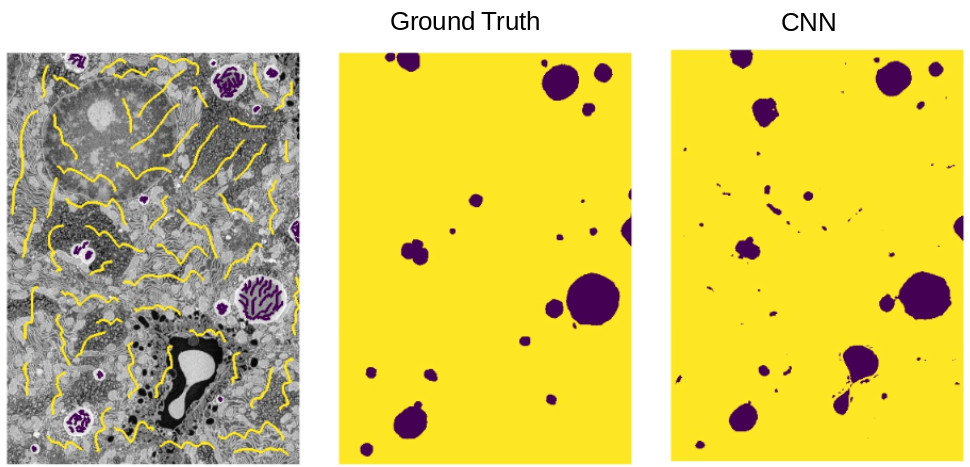
\includegraphics[width=1.0\linewidth]{figures/cnn1.jpeg} 
\caption{Segmentation mask generated using OSVOS and $\mathcal{L}_{\rm{scribble}}$. Left-most image shows foreground (violet) and background (yellow) scribbles}
\end{figure}

We can observe that using significant amout of scribbles CNN is able to learn the shape of object. As we manually annotated some pixels in each vesicle for the slice in figure 4.1, the CNNs are able to segment all vesicles. The accuracy gets limited by the amount of false positives. We can observe that for a lot of background pixels which are not annotated as background scribbles for training, the CNN predicts them as foreground pixels in output mask. This happens mainly for the pixels which are similar to foreground pixels in terms of pixel intensity. In addition to these pixels, we can see some noisy pixels predicted as foreground. This motivated us to make use of prior and clear this mask using variational image processing. \par
To compare the results and accuracy of CNN and VIP for different annotation budgets, we repeated the experiment done for RF using "easy" and "hard" scribbles, explained in section 3.2.1. Similar to experiment in RF, we trained the CNN by first adding annotations from "easy" scribbles and then, from "hard" scribbles. We take the original pre-trained parent OSVOS network and fine-tune it using scribbles. Each time we add new scribbles, we fine-tune the parent OSVOS network and test the network on the same image. Similar to section 3.3, we use probability mask predicted from CNN to compute anti-loglikelihood cost function and estimate a mask using equation 3.3. For results (shown in figure 4.2) using CNN, we make use of only anti-loglikelihood cost function.

\begin{figure}[h!] \label{fig:cnnvip}
\centering
 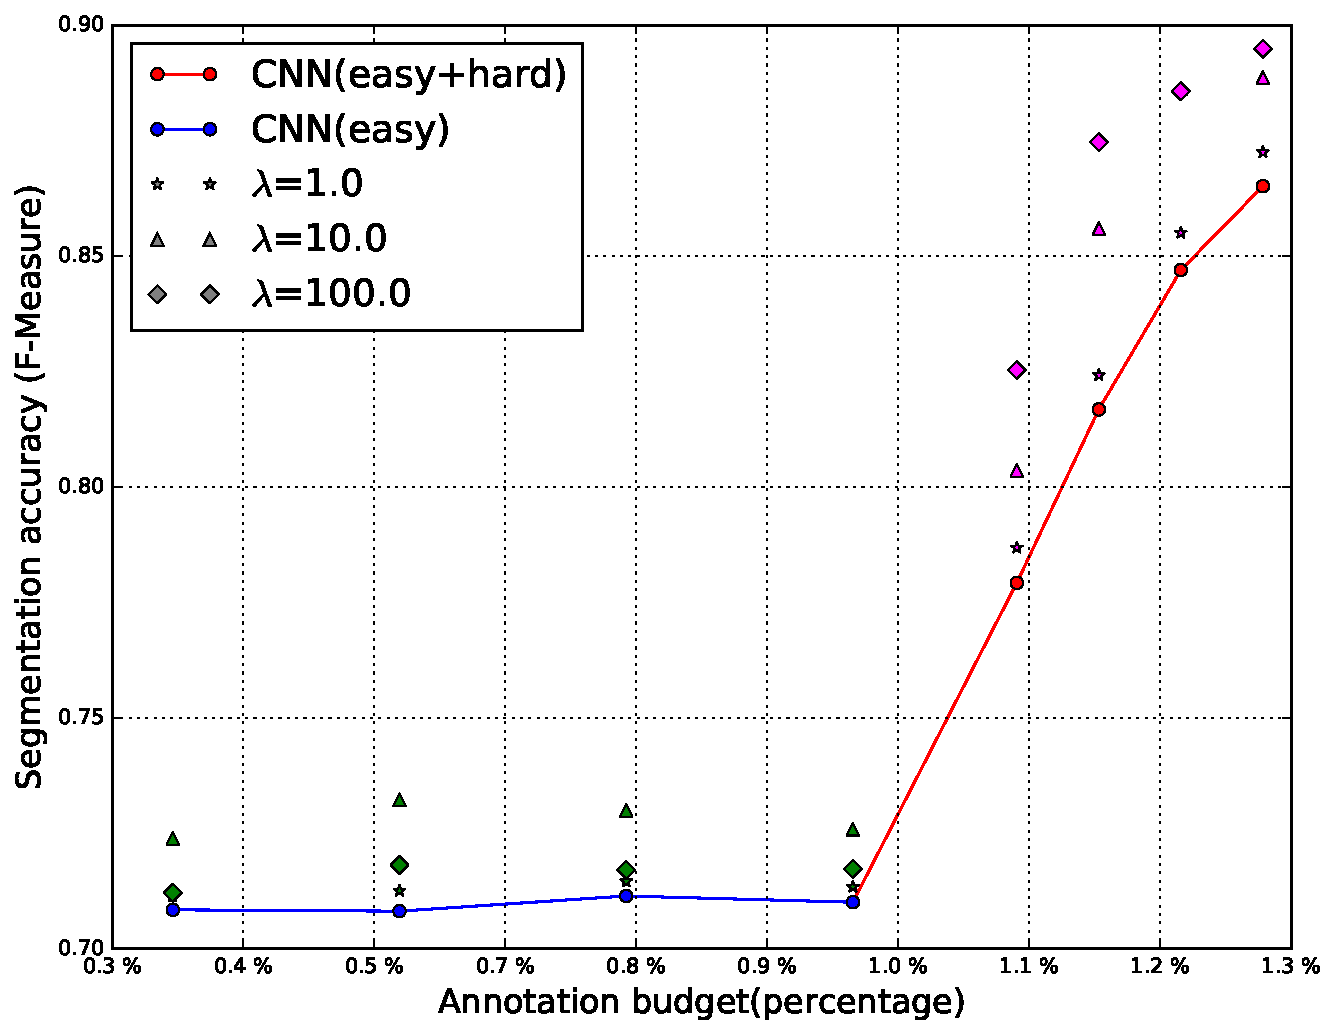
\includegraphics[width=0.8\linewidth]{figures/cnn_vip.pdf}
 \caption{Segmentation accuracy for CNN with VIP (different $\lambda$)}
\end{figure}

Using around only 0.35\% of total pixels, we are able to achieve an accuracy of 0.72.
Although, when CNN is trained using full annotations, it is expected to produce highly accurate results and do not improve with use of VIP. But, here, the accuracy imporves with the use of VIP for all annotation budgets. We are able to achieve this improvement without significant addition to computational cost. Similar to RF, the addition of "hard" scribbles (red curve in figure 4.2), the accuracy starts improving with a jump. Next, we compare the results from RF and CNN. We use the same amount of scribbles for "easy" and "hard" annotation class and make a comarison of results in figure 4.3.  

\begin{figure}[h!] \label{fig:cnnvip}
\centering
 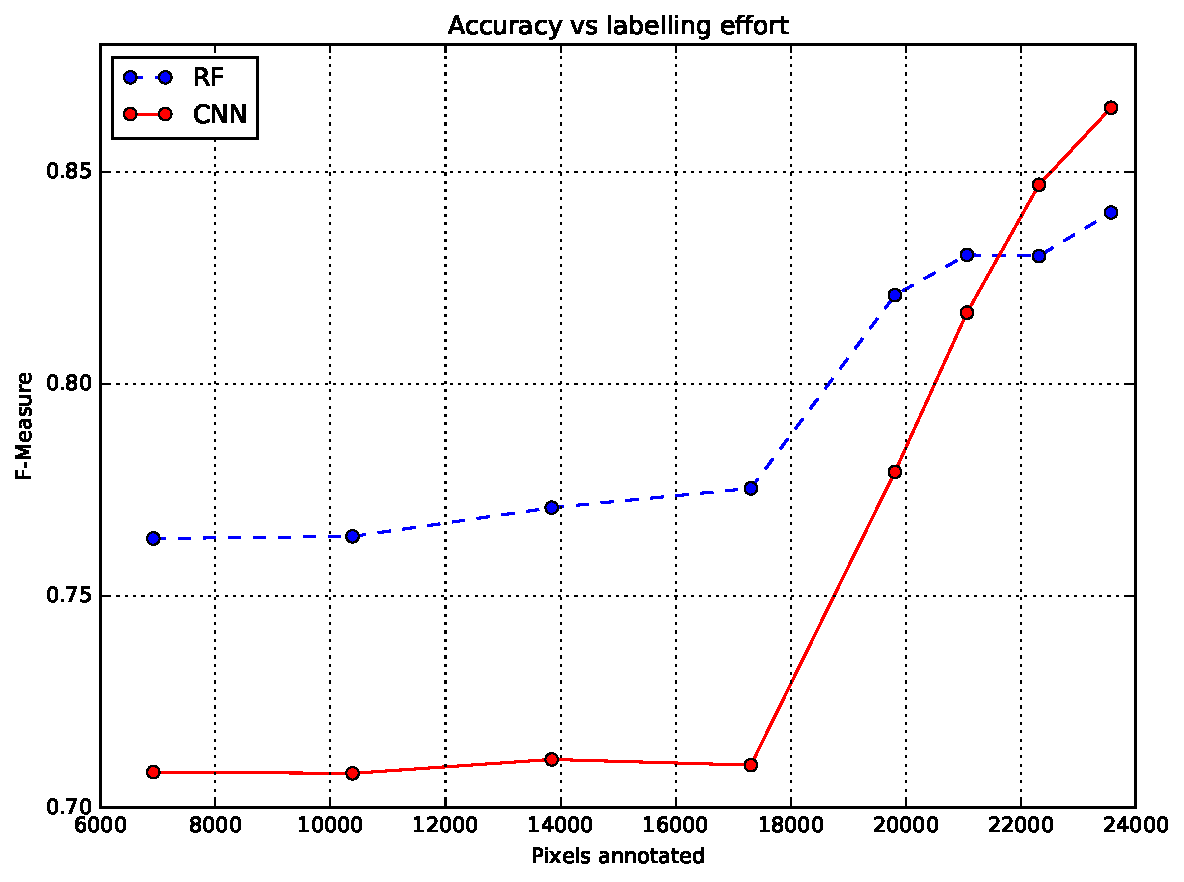
\includegraphics[width=0.8\linewidth]{figures/cnn_vs_rf.pdf} 
\caption{Segmentation accuracy for mask obtained from RF and CNN, after thresholding}
\end{figure}

For lower annotation budgets in our segmentation task, RF performs significantly better than CNN. We can expect this for CNN due to significantly less training data. The weights and biases in multiple layers of OSVOS are not able to adapt much and converge properly. But as the annotation budget becomer more than 1.2\%, the CNN outperforms RF. With significant amount of scribbles, it also tries to learn the shape and the size of vesicles. The CNN is able to achieve a segmentation accuracy of 0.86 with only 1.3\% of pixels used for training. Also, the intersection (red and blue curve in figure 4.3) can be seen as a boundary to choose RF or CNN for a given annotation budget. \par

Finally, we compare the results of RF and CNN in a Bayesian framework. Using the masks obtained from RF and CNN for a certain annotation budget, we use VIP to obtain an optimal mask. The results is figure 4.4 show improvement for different $\lambda$. For annotation budget of around 1.3\% and use of VIP, RF is able to achieve accuracy close to that obtained from CNN and VIP. 


\begin{figure}[h!] \label{fig:cnnvip}
\centering
 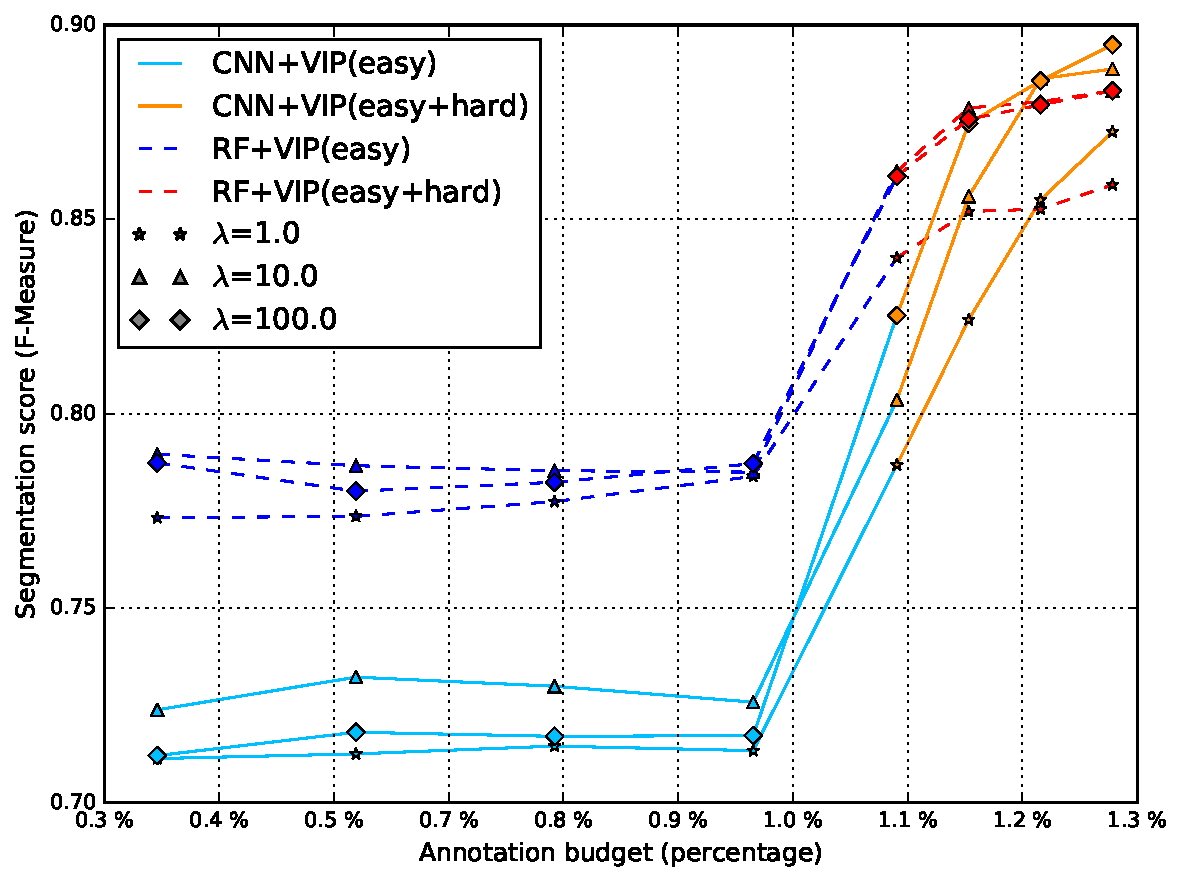
\includegraphics[width=0.8\linewidth]{figures/cnn_vs_rf_vip.pdf} 
\caption{Segmentation accuracy for mask obtained from RF and CNN, both with VIP}
\end{figure}
